\documentclass[a4paper,11pt]{article}
\usepackage{a4wide}
\usepackage{fullpage}
\usepackage[utf8x]{inputenc}
%\usepackage[slovene]{babel}
%\selectlanguage{slovene}
\usepackage[toc,page]{appendix}
\usepackage[pdftex]{graphicx} 
\usepackage{amsfonts}
\usepackage{amsmath}
\usepackage{setspace}
\usepackage{color}
\definecolor{light-gray}{gray}{0.95}
\usepackage{listings} 
\usepackage{hyperref}
\renewcommand{\baselinestretch}{1.2} 
\renewcommand{\appendixpagename}{Priloge}

\lstset{ 
language=Python,
basicstyle=\footnotesize,
basicstyle=\ttfamily\footnotesize\setstretch{1},
backgroundcolor=\color{light-gray},
}

\title{Topological data analysis \\ Homework 1}
\author{Sara Bizjak (27202020)}
\date{\today}

\begin{document}

\maketitle

\section{Theoretical problems}
\subsection{Exploring different metrics}

%%%%%%%%%%%%%%%%%%%%%%%%%%%%%%%%%%%%%%%%%%%%%%%%%%%%%%%%%%%%%%%%%%%%%%%%%%%%%%%%

a) Determing the distances between the points $(2, 1), \ (4, 2), \ (0, 2)$ in metrics $\alpha, \  \beta, \ \gamma$.

\begin{itemize}
    \item Metric $\alpha$.
        
    \begin{equation*}
        \text{d}_{\alpha} \big( (2, 1), \ (4, 2) \big) = \sqrt{2^2 + 1^2} + \sqrt{4^2 + 2^2} = \sqrt{5} + \sqrt{20} = 6.708203932499369.
    \end{equation*}

    \begin{equation*}
        \text{d}_{\alpha} \big( (2, 1), \ (0, 2) \big) = \sqrt{2^2 + 1^2} + \sqrt{0^2 + 2^2} = \sqrt{5} + \sqrt{4} = 4.23606797749979.
    \end{equation*}

    \begin{equation*}
        \text{d}_{\alpha} \big( (4, 2), \ (0, 2) \big) = \sqrt{4^2 + 2^2} + \sqrt{0^2 + 2^2} = \sqrt{20} + \sqrt{4} = 6.47213595499958.
    \end{equation*}

%%%%%%%%%%%%%%%%%%%%%%%%%%%%%%%%%%%%%%%%%

    \item Metric $\beta$.
    
    \begin{equation*}
        \text{d}_{\beta} \big( (2, 1), \ (4, 2) \big) = \sqrt{(2 - 4)^2 + (1 - 2)^2} = \sqrt{4 + 1} = 2.23606797749979.
    \end{equation*}
        
    \begin{equation*}
        \text{d}_{\beta} \big( (2, 1), \ (0, 2) \big) = \sqrt{2^2 + 1^2} + \sqrt{0^2 + 2^2} = \sqrt{5} + \sqrt{4} = 4.23606797749979.
    \end{equation*}
        
    \begin{equation*}
        \text{d}_{\beta} \big( (4, 2), \ (0, 2) \big) = \sqrt{4^2 + 2^2} + \sqrt{0^2 + 2^2} = \sqrt{20} + \sqrt{4} = 6.47213595499958.
    \end{equation*}

%%%%%%%%%%%%%%%%%%%%%%%%%%%%%%%%%%%%%%%%%

    \item Metric $\gamma$.
    
    \begin{equation*}
        \text{d}_{\gamma} \big( (2, 1), \ (4, 2) \big) = |2 - 4| + |1| + |2| = 2 + 1 + 2 = 5.
    \end{equation*}
        
    \begin{equation*}
        \text{d}_{\gamma} \big( (2, 1), \ (0, 2) \big) = |2 - 0| + |1| + |2| = 5.
    \end{equation*}
        
    \begin{equation*}
        \text{d}_{\gamma} \big( (4, 2), \ (0, 2) \big) = |4 - 0| + |2| + |2| = 4 + 2 + 2 = 8.
    \end{equation*}


\end{itemize}

%%%%%%%%%%%%%%%%%%%%%%%%%%%%%%%%%%%%%%%%%%%%%%%%%%%%%%%%%%%%%%%%%%%%%%%%%%%%%%%%

b) Draw the open balls $B \big((0, 0), 1 \big)$, $B \big((1, 0), 2 \big)$, $B \big((0, 2), 6 \big)$ in $\alpha$ metric. 

\begin{align*} 
    B \big((0, 0), 1 \big) &= \{(0,0)\} \cup \{(x,y) \in \mathbb{R}^2 : \sqrt{x^2 + y^2} + \sqrt{0^2 + 0^2}< 1 \} 
    \\
    &= \{(0,0)\} \cup \{(x,y) \in \mathbb{R}^2 : \sqrt{x^2 + y^2} < 1 \}. 
\end{align*}

\begin{figure}[ht!]
    \centering
    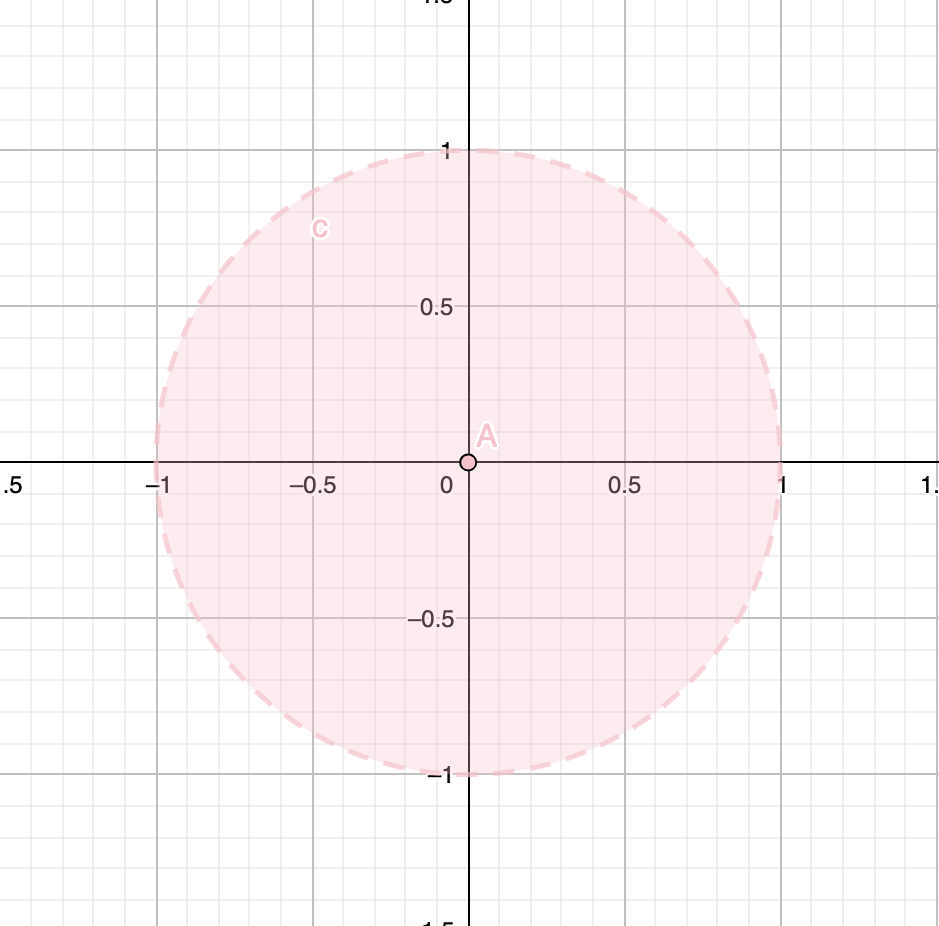
\includegraphics[width=60mm]{b1.png}
    \caption{$B \big((0, 0), 1 \big)$ in metric $\alpha$.}
\end{figure}

%%%%%%%%%%%%%%%%%%%%%%%%%%%%%%%%%%%%%%%%%%

\begin{align*} 
    B \big((1, 0), 2 \big) &= \{(1,0)\} \cup \{(x,y) \in \mathbb{R}^2 \setminus (1,0) : \sqrt{x^2 + y^2} + \sqrt{1^2 + 0^2} < 2 \}
    \\
    &= \{(1,0)\} \cup \{(x,y) \in \mathbb{R}^2 \setminus (1,0) : \sqrt{x^2 + y^2} < 1 \} .
\end{align*}

\begin{figure}[ht!]
    \centering
    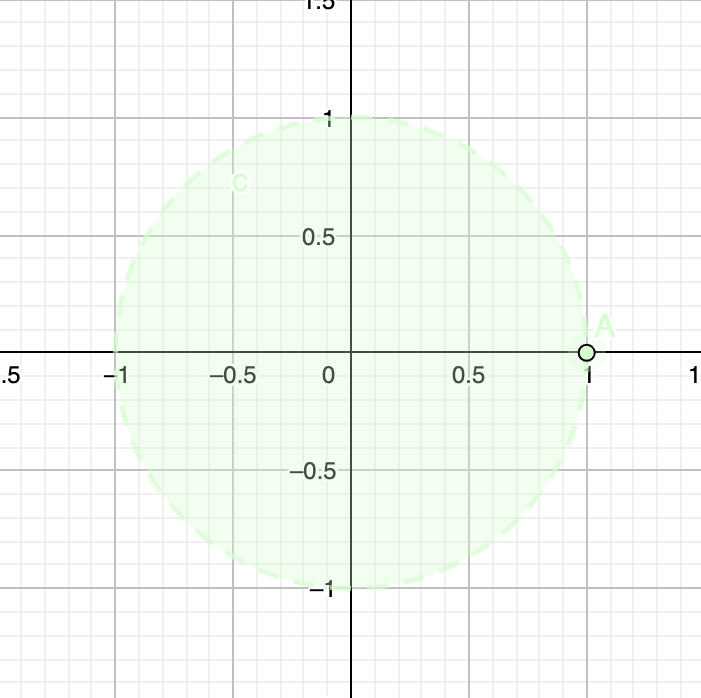
\includegraphics[width=60mm]{b2.png}
    \caption{$B \big((1, 0), 2 \big)$ in metric $\alpha$.}
\end{figure}

 %%%%%%%%%%%%%%%%%%%%%%%%%%%%%%%%%%%%%%%%%

 \begin{align*} 
    B \big((0, 2), 6 \big) &= \{(0,2)\} \cup \{(x,y) \in \mathbb{R}^2 \setminus (0,2) : \sqrt{x^2 + y^2} + \sqrt{0^2 + 2^2} < 6 \} 
    \\
    &= \{(0,2)\} \cup \{(x,y) \in \mathbb{R}^2 \setminus (0,2) : \sqrt{x^2 + y^2} < 4 \}. 
\end{align*}

\begin{figure}[ht!]
    \centering
    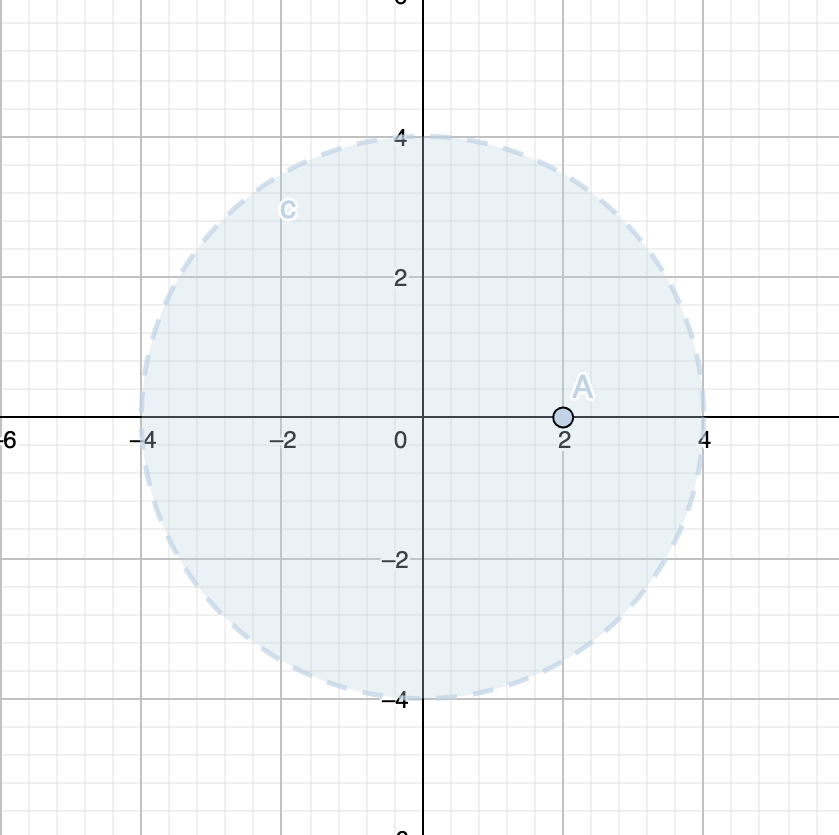
\includegraphics[width=60mm]{b3.png}
    \caption{$B \big((0, 2), 6 \big)$ in metric $\alpha$.}
\end{figure}
%%%%%%%%%%%%%%%%%%%%%%%%%%%%%%%%%%%%%%%%%%%%%%%%%%%%%%%%%%%%%%%%%%%%%%%%%%%%%%%%%%%%%%

c) Draw the open balls $B \big((0, 0), 1 \big)$, $B \big((1, 0), 2 \big)$, $B \big((2, 2), 3 \sqrt{2} \big)$ in $\beta$ metric. 

\begin{align*} 
    B \big((0, 0), 1 \big) &= \{(x,y) \in \mathbb{R}^2 : \sqrt{(x - 0)^2 + (y - 0)^2} < 1 \}
    \\
    &= \{(x,y) \in \mathbb{R}^2 : \sqrt{x^2 + y^2} < 1 \}.
\end{align*}

\begin{figure}[ht!]
    \centering
    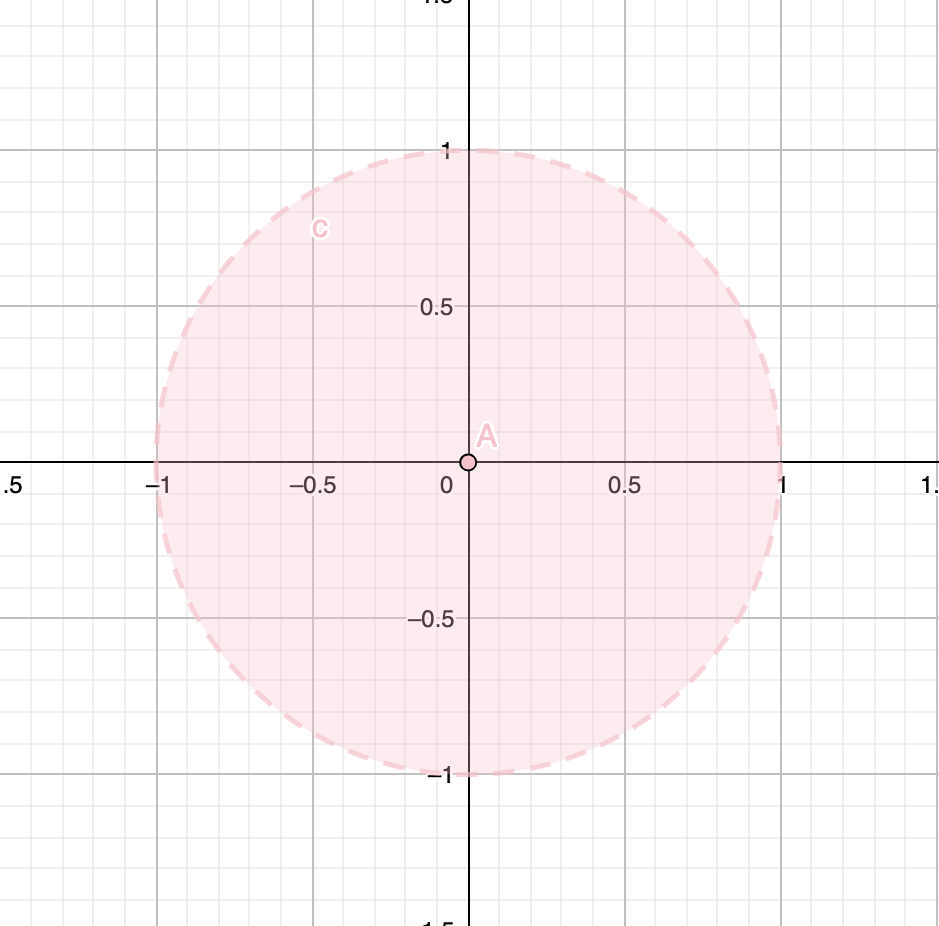
\includegraphics[width=60mm]{b1.png}
    \caption{$B \big((0, 0), 1 \big)$ in metric $\beta$.}
\end{figure}

%%%%%%%%%%%%%%%%%%%%%%%%%%%%%%%%%%%%%%%%%%%%

\begin{align*} 
    B \big((1, 0), 2 \big) &= \{(x,0) \in \mathbb{R}^2 : \sqrt{(x - 1)^2} < 2 \} \cup \{(x, y) \in \mathbb{R}^2, \ y \neq 0 : \sqrt{x^2 + y^2} + \sqrt{1^2} < 2 \}
    \\
    &= \{(x,0) \in \mathbb{R}^2 : |x - 1| < 2 \} \cup \{(x,y) \in \mathbb{R}^2, \ y \neq 0 : \sqrt{x^2 + y^2} < 1 \} 
    \\
    &= \{(x,0) \in \mathbb{R}^2 : -1 < x < 3 \} \cup \{(x,y) \in \mathbb{R}^2, \ y \neq 0 : \sqrt{x^2 + y^2} < 1 \} .
\end{align*}

\begin{figure}[ht!]
    \centering
    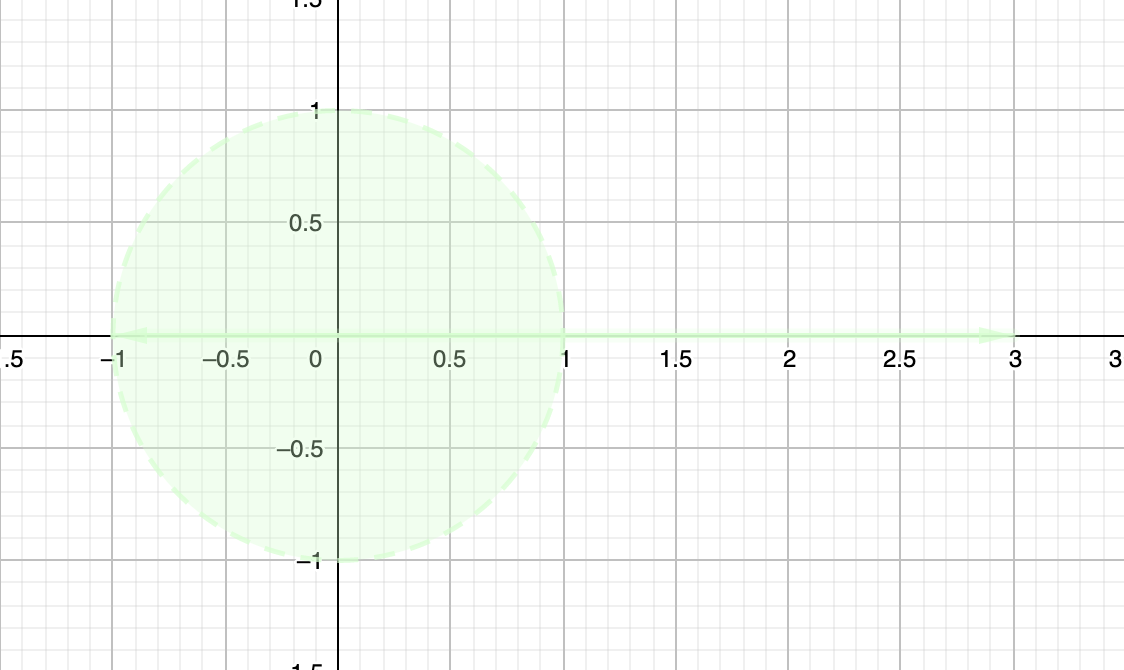
\includegraphics[width=60mm]{c2.png}
    \caption{$B \big((1, 0), 2 \big)$ in metric $\beta$.}
\end{figure}

 %%%%%%%%%%%%%%%%%%%%%%%%%%%%%%%%%%%%%%%%%%%

\begin{align*} 
    B \big((2, 2), 3 \sqrt{2} \big) &= \{(x,x) \in \mathbb{R}^2 : \sqrt{2 \cdot (x - 2)^2} < 3 \sqrt{2} \} \cup \{(x, y) \in \mathbb{R}^2, \ x \neq y : \sqrt{x^2 + y^2} + \sqrt{2 \cdot 2^2} < 3 \sqrt{2} \}
    \\
    &= \{(x,x) \in \mathbb{R}^2 : \sqrt{2} \cdot |x - 2| < 3 \sqrt{2} \} \cup \{(x,y) \in \mathbb{R}^2, \ x \neq y : \sqrt{x^2 + y^2} + 2 \sqrt{2} < 3 \sqrt{2} \} 
    \\
    &= \{(x,x) \in \mathbb{R}^2 : -1 < x < 5\} \cup \{(x,y) \in \mathbb{R}^2, \ x \neq y : \sqrt{x^2 + y^2} < \sqrt{2} \} .
\end{align*}

\begin{figure}[ht!]
    \centering
    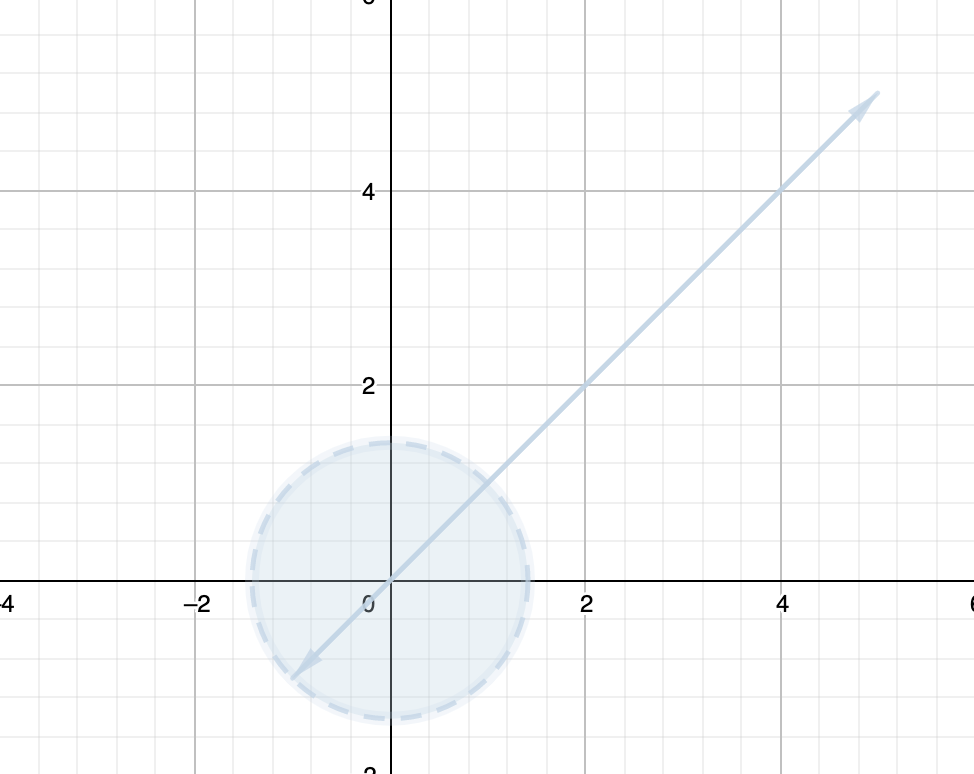
\includegraphics[width=60mm]{c3.png}
    \caption{$B \big((2, 2), 3 \sqrt{2} \big)$ in metric $\beta$.}
\end{figure}

%%%%%%%%%%%%%%%%%%%%%%%%%%%%%%%%%%%%%%%%%%%%%%%%%%%%%%%%%%%%%%%%%%%%%%%%%%%%%%%%%%%%%%%%%%%%%

d) Draw the open balls $B \big((0, 0), 1 \big)$, $B \big((1, 0), 2 \big)$, $B \big((2, 0), 3  \big)$ in $\gamma$ metric. 

\begin{align*} 
    B \big((0, 0), 1 \big) &= \{(0,y) \in \mathbb{R}^2 : |y - 0| < 1 \} \cup \{(x,y) \in \mathbb{R}^2 , \ x \neq 0: |x - 0| + |y - 0| < 1 \}
    \\
    &= \{(0,y) \in \mathbb{R}^2 : -1 < y < 1 \} \cup \{(x,y) \in \mathbb{R}^2 : -1 < x < 1, \ -1 < y < 1 \}.
\end{align*}

\begin{figure}[ht!]
    \centering
    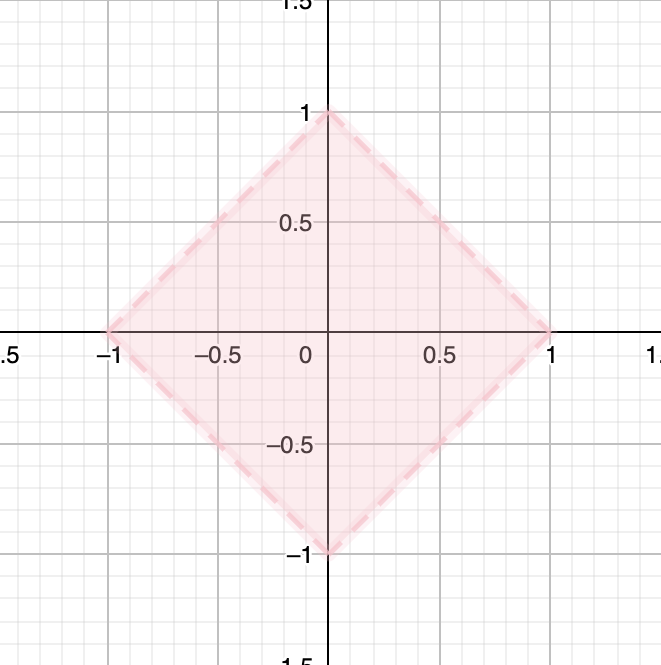
\includegraphics[width=60mm]{d1.png}
    \caption{$B \big((0, 0), 1 \big)$ in metric $\gamma$.}
\end{figure}

%%%%%%%%%%%%%%%%%%%%%%%%%%%%%%%%%%%%%%%%%%%%
\begin{align*} 
    B \big((1, 0), 2 \big) &= \{(1,y) \in \mathbb{R}^2 : |y - 0| < 2 \} \cup \{(x,y) \in \mathbb{R}^2, \ x \neq 1 : |x - 1| + |y - 0| < 2 \}
    \\
    &= \{(1,y) \in \mathbb{R}^2 : -2 < y < 2 \} \cup \{(x,y) \in \mathbb{R}^2 , \ x \neq 1: -1 < x < 3, \ -2 < y < 2 \}.
\end{align*}

\begin{figure}[ht!]
    \centering
    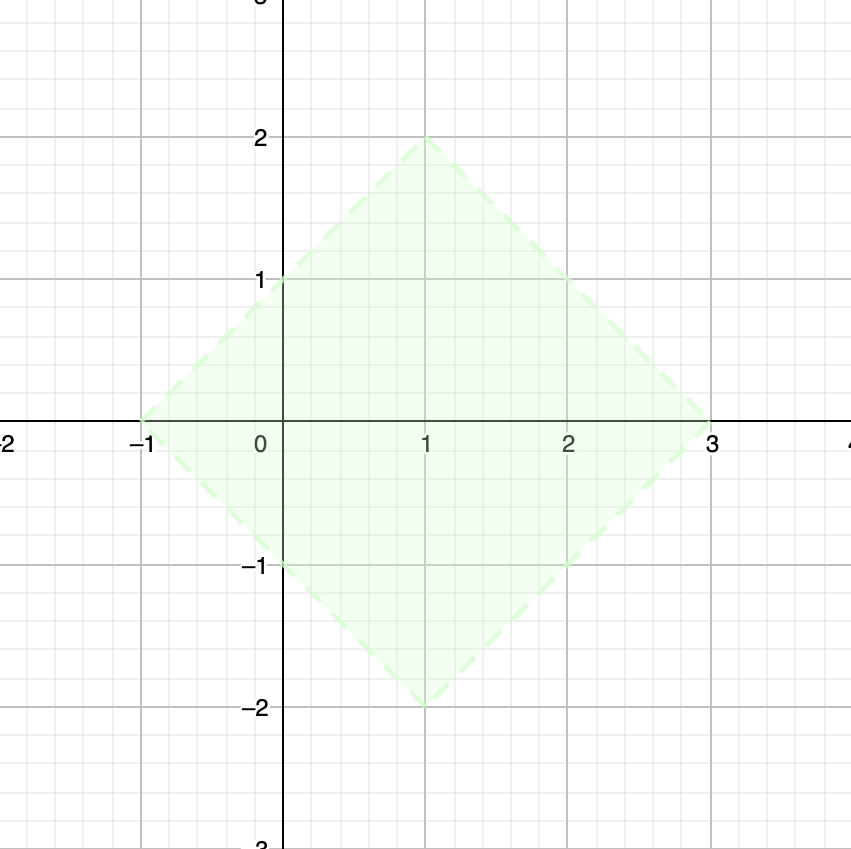
\includegraphics[width=60mm]{d2.png}
    \caption{$B \big((1, 0), 2 \big)$ in metric $\gamma$.}
\end{figure}

 %%%%%%%%%%%%%%%%%%%%%%%%%%%%%%%%%%%%%%%%%%%
\begin{align*} 
    B \big((2, 0), 3 \big) &= \{(2,y) \in \mathbb{R}^2 : |y - 0| < 3 \} \cup \{(x,y) \in \mathbb{R}^2, \ x \neq 2 : |x - 2| + |y - 0| < 3 \}
    \\
    &= \{(2,y) \in \mathbb{R}^2 : -3 < y < 3 \} \cup \{(x,y) \in \mathbb{R}^2 , \ x \neq 2: -1 < x < 5, \ -3< y < 3 \}.
\end{align*}

\begin{figure}[ht!]
    \centering
    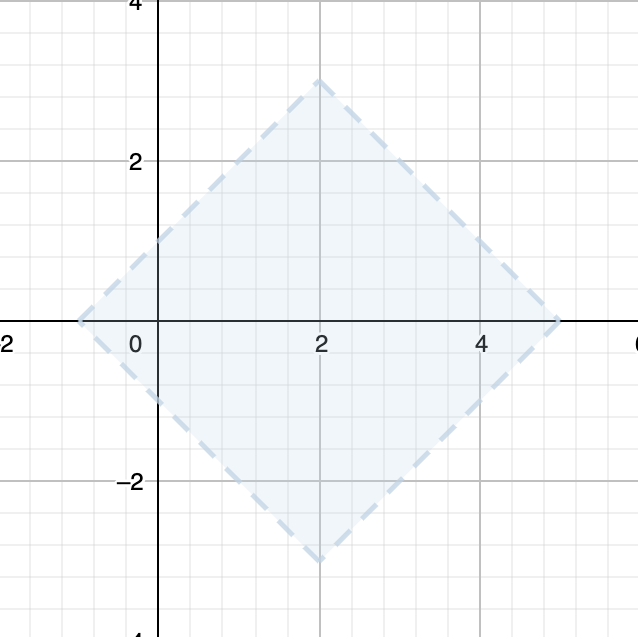
\includegraphics[width=60mm]{d3.png}
    \caption{$B \big((2, 0), 3 \big)$ in metric $\gamma$.}
\end{figure}



%%%%%%%%%%%%%%%%%%%%%%%%%%%%%%%%%%%%%%%%%%%%%%%%%%%%%%%%%%%%%%%%%%%%%%%%%%%%%%%%%%%%%%%%%%%%%%%%%%%%%%%%%%%%%%%%%%%%%%%%%%%%%%%%%%%%%%%%%%%%%%%%%%%%%%%%%%%%%%%%%%%%%%%%%%%%%%%%

\newpage
\subsection{Discrete metric}
The discrete metric on a space $X$ is defined as $d: \ X \times X \to \mathbb{R}$, where $d(x, y) = 1$ if $x = y$ and $1$ otherwise.

\noindent
a) Let $X = \mathbb{N}$. Describe $B \big(1, \frac{1}{2} \big)$ and $B \big(2, 1 \big)$.

\begin{center}
$ B \left(1, \frac{1}{2} \right) = \{ x \in \mathbb{N} : d(1, x) < \frac{1}{2} \} = \{ x = 1 : d(1, 1) = 0 \} = {1}. $
\\
$ B (2, 1) = \{ x \in \mathbb{N} : d(2, x) < 1 \} = \{ x = 2 : d(2, 2) = 0 \} = {2}. $
\\
\end{center}

%%%%%%%%%%%%%%%%%%%%%%%%%%%%%%%%%%%

\noindent
b) The triangle with vertices at distinct integers $a, b, c$ is always equilateral, because the distance between distinct points in discrete metric is always $1$.

%%%%%%%%%%%%%%%%%%%%%%%%%%%%%%%%%%%%%%%%%%%%%%%%%%%%%%%%%%%%%%%%%%%%%%%%%%%%%%%%%%%%%%%%%%%%%%%%%%%%%%%%%%%%%%%%%%%%%%%%%%%%%%%%%%%%%%%%%%%%%%%%%%%%%%%%%%%%%%%%%%%%%%%%%%%%%%%%

\subsection{Homeomorphic spaces}

Let $X = S^{n - 1} \times [0,1] \subset \mathbb{R}^{n+1}$ and $Y = \{ (x_1, \ldots, x_n) \in \mathbb{R}^n \ : \ 1 \leq x_1^2 + \cdots + x_n^2 \leq 4 \}$. What we want to do is to prove that $X$ and $Y$ are homeomorphic.
Therefore, we need to define continuous functions $f: X \to Y$ and $g: Y \to X$ and show that $g = f^{-1}$. We do that by calculating $f \circ g $ and $g \circ f$ and show that they are identities.
\\
To get an idea, we first look at the sketches of spaces $X$ and $Y$ for $n = 1$ and $n = 2$, denoted as $X_1, X_2$ and $Y_1, Y_2$.
\\

\begin{figure}[ht!]
     \begin{minipage}{0.5\textwidth}
         \centering
         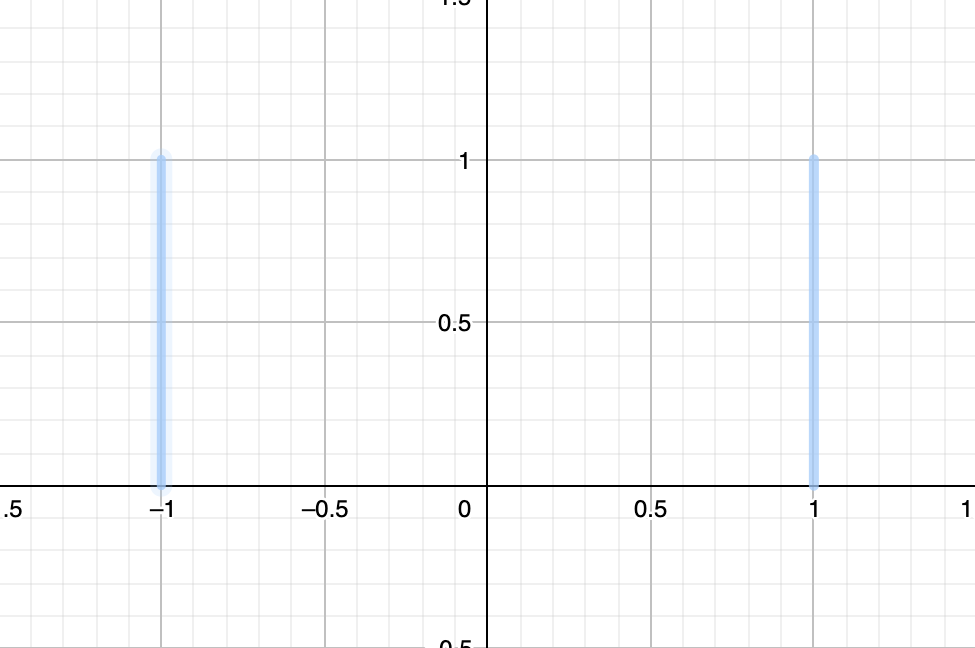
\includegraphics[width=50mm]{X_n1.png}
         \caption{$X_1 = S^0 \times [0,1] \subset \mathbb{R}^2$.}
       \end{minipage}\hfill
     \begin{minipage}{0.5\textwidth}
         \centering
         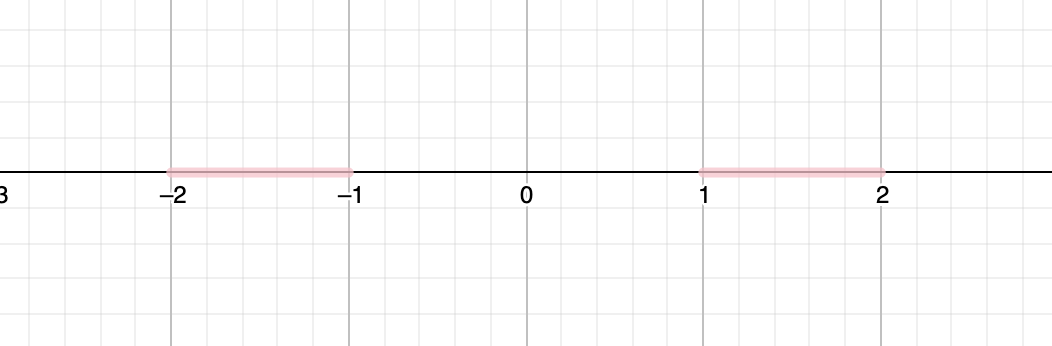
\includegraphics[width=70mm]{Y_n1.png}
         \caption{$ Y_1 = \{ x_1 \in \mathbb{R} : 1 \leq x_1^2 \leq 4 \}$.}
       \end{minipage}\hfill
    \end{figure}

\begin{figure}[ht!]
     \begin{minipage}{0.45\textwidth}
         \centering
         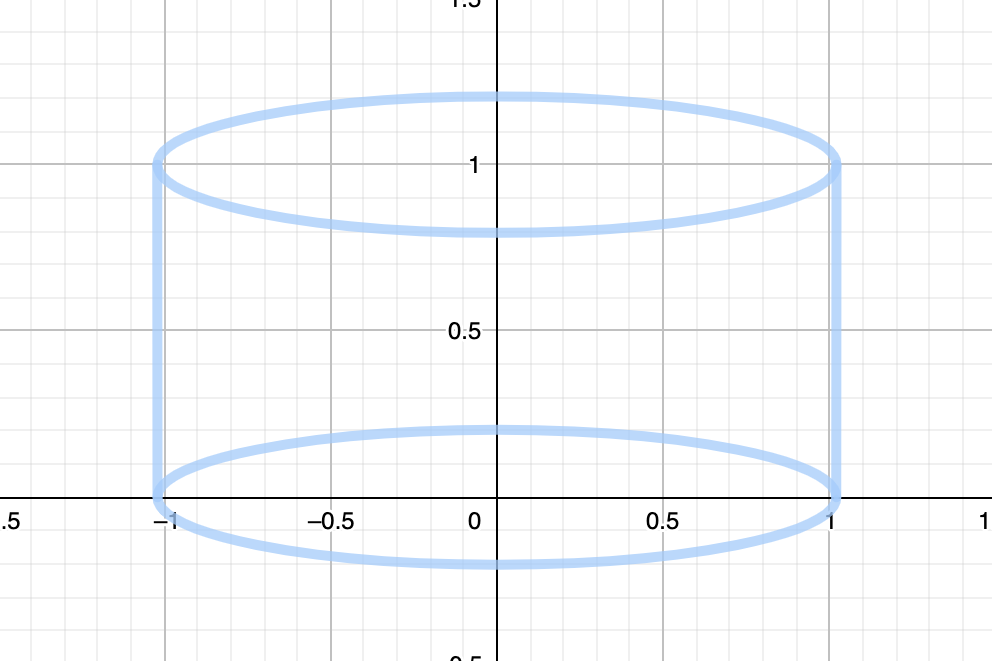
\includegraphics[width=50mm]{X_n2.png}
         \caption{$X_2 = S^1 \times [0,1] \subset \mathbb{R}^3$.}
       \end{minipage}\hfill
     \begin{minipage}{0.55\textwidth}
         \centering
         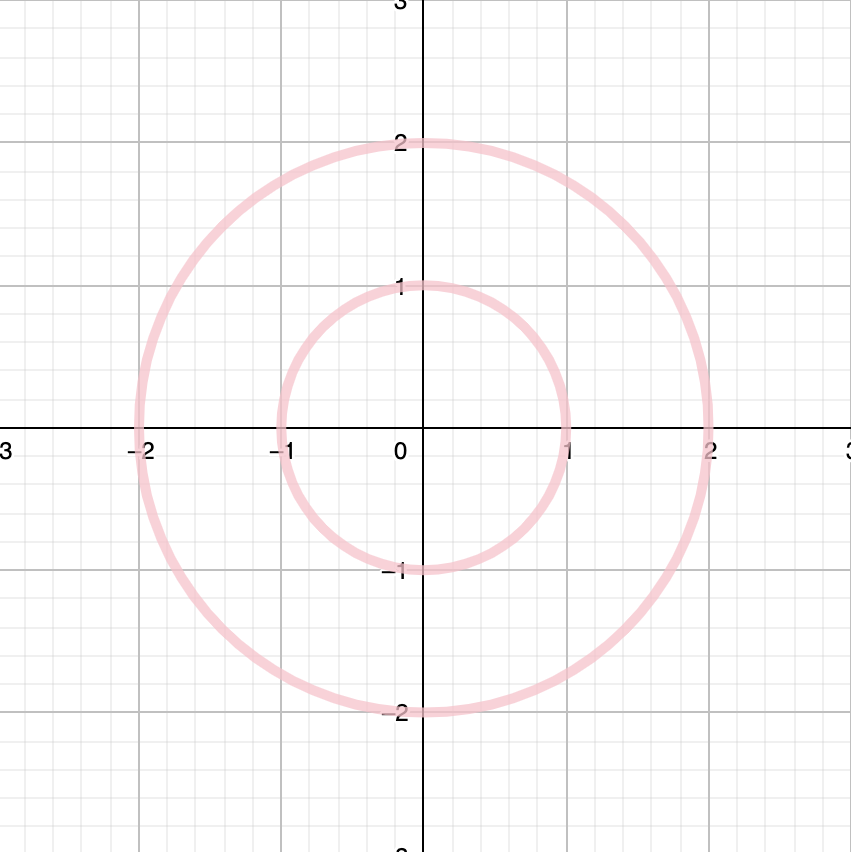
\includegraphics[width=50mm]{Y_n2.png}
         \caption{$ Y_2 = \{ (x_1, x_2) \in \mathbb{R}^2 : 1 \leq x_1^2 + x_2^2 \leq 4 \}$.}
       \end{minipage}\hfill
    \end{figure}

\newpage
\noindent
We imagine space $X_2$ as an union of disjointed lines connecting upper and lower circle edges. Similarly, we imagine space $Y_2$. Let's present this idea in the following pictures.

\begin{figure}[ht!]
    \begin{minipage}{0.45\textwidth}
        \centering
        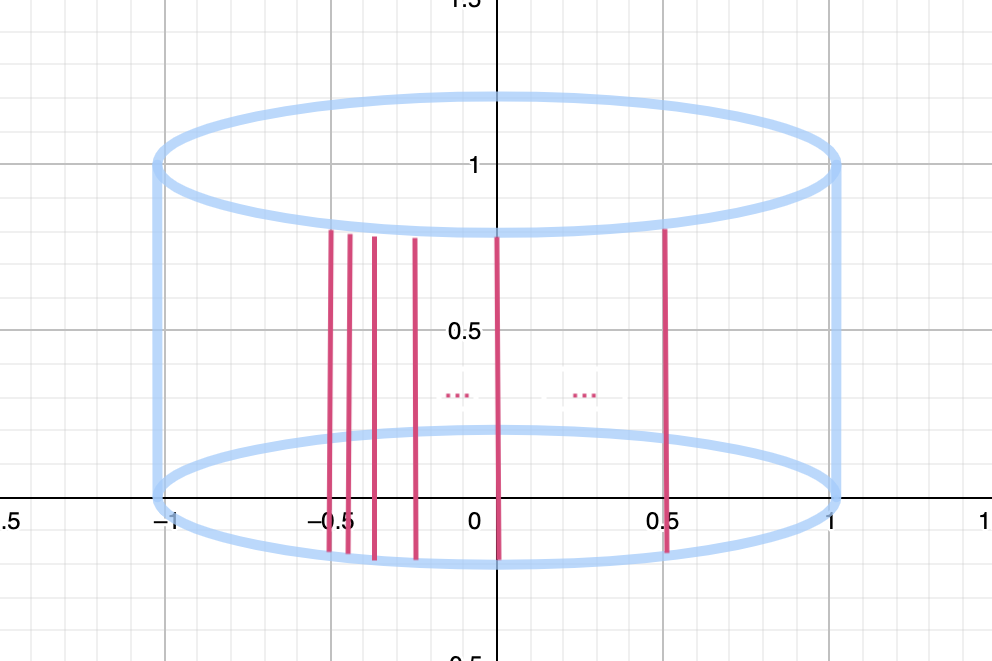
\includegraphics[width=60mm]{X_n2_lines.png}
        \caption{$X_2$ as an union of disjoint lines.}
      \end{minipage}\hfill
    \begin{minipage}{0.55\textwidth}
        \centering
        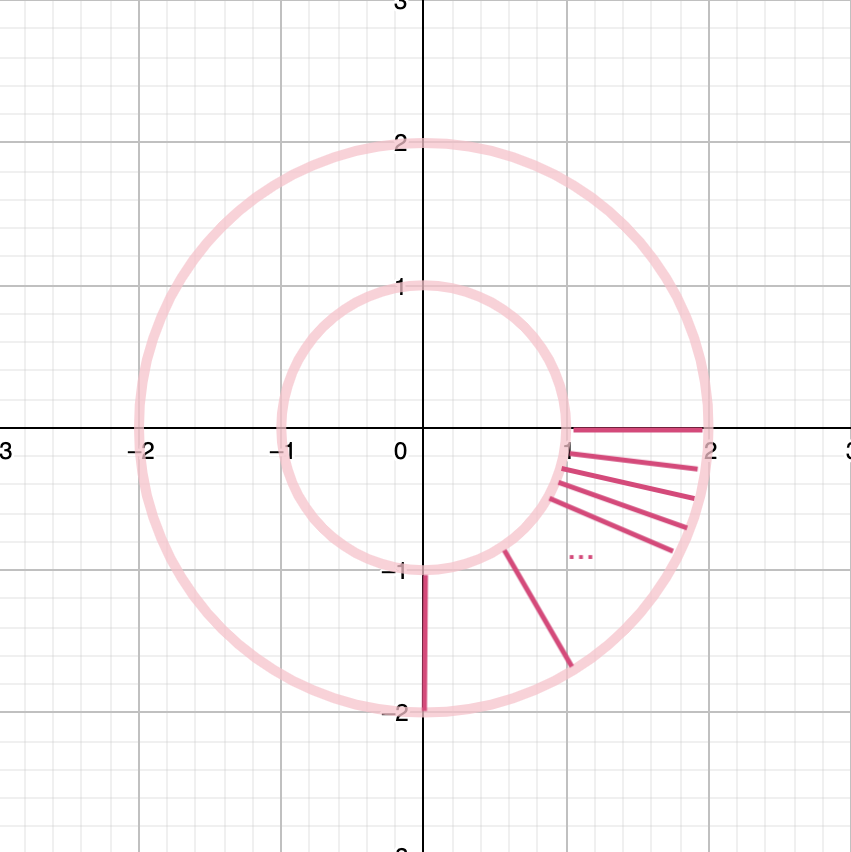
\includegraphics[width=60mm]{Y_n2_lines.png}
        \caption{$Y_2$ as an unoin of disjoint lines.}
      \end{minipage}\hfill
   \end{figure}

\noindent
We see that we can go from space $X_2$ to space $Y_2$ by "flipping" lines down on the plane. And equivalently, from $Y_2$ to $X_2$ we do the same thing but in reverse.
\\
Lines in $X_2$ have the form of $(1 - t) \cdot (x_1, x_2, 0) + t \cdot (x_1, x_2, 1)$ and lines in $Y_2$ have the form of $(1 - t) \cdot (x_1, x_2) + 2  t \cdot (x_1, x_2)$, where $ t \in [0, 1]$.
\\
To get from $X_2$ to $Y_2$ we have to project lines to $x_1 x_2-$plane (by skipping the third coordinate) and then stretch them with factor  $(1 + t)$, where $t \in [0,1]$.
On the other hand, to get from $Y_2$ to $X_2$ we have to squeeze the lines to the unit circle (normalization) and then stretch them up from $0$ to $1$, so we write the new coordinate, denoted by t, as a function of $x_1$ and $x_2$.
Following this idea, functions $f_2: X_2 \to Y_2$ and $g_2: Y_2 \to X_2$ are: \\
$f_2(x_1, x_2, t) = (x_1 \cdot (1 + t), x_2 \cdot (1 + t))$ \ and \
$g_2(x_1, x_2) = \left( \frac{x_1}{\sqrt{x_1^2 + x_2^2}}, \frac{x_2}{\sqrt{x_1^2 + x_2^2}}, \sqrt{x_1^2 + x_2^2} - 1 \right),$  where $t \in [0,1]$.
\\
\\
Let's get back to $X$ and $Y$ spaces and use our idea for general n.
Let $f: X \to Y$ and let $g: Y \to X$. Function $f$ is:

$$ f(x_1, \ldots, x_n, t) =  \left( x_1 \cdot (1 + t), \ldots, x_n \cdot (1 + t) \right) = (1 + t) \cdot (x_1, \ldots, x_n). $$

\noindent
Now, we need to verify that $(1 + t) \cdot (x_1, \ldots, x_n) \in Y$. Because $(x_1, \ldots, x_n, t) \in X$, then $x_1^2 + \cdots + x_n^2 = 1$ and $t \in [0,1]$.
So $((1 + t) \cdot x_1)^2 + \cdots + ((1 + t) \cdot x_2)^2 = (1 + t)^2 \cdot (x_1^2 + \cdots + x_n^2)^2 = (1 + t)^2$ and $1 \leq (1 + t)^2 \leq 4$, so the condition is satisfied.
\\
\\
For function $g$ we need to express the new coordinate $t$ as a function of $(x_1, \ldots, x_n)$. For $t \in [0, 1]$ the relation $t = \sqrt{x_1^2 + \cdots x_n^2} - 1 $ is obvious. 
$$ g(x_1, \ldots, x_n) = \left( \frac{x_1}{ \sqrt{x_1^2 + \cdots + x_n^2}}, \ldots, \frac{x_n}{ \sqrt{x_1^2 + \cdots + x_n^2}}, \sqrt{x_1^2 + \cdots + x_n^2} - 1 \right). $$ 
\noindent
Similarly as we did for function $f$, we now need to verify that \\
$ \left( \frac{x_1}{ \sqrt{x_1^2 + \cdots + x_n^2}}, \ldots, \frac{x_n}{ \sqrt{x_1^2 + \cdots + x_n^2}}, \sqrt{x_1^2 + \cdots + x_n^2} - 1 \right) \in X$.
Because $(x_1, \ldots, x_n) \in Y$ follows  $1 \leq x_1^2 + \cdots + x_n^2 \leq 4$. Since $\left( \frac{x_1}{ \sqrt{x_1^2 + \cdots + x_n^2}} \right)^2 + \cdots + \left( \frac{x_n}{ \sqrt{x_1^2 + \cdots + x_n^2}} \right)^2 = \frac{x_1^2 + \cdots + x_n^2}{x_1^2 + \cdots + x_n^2} = 1$ and $t = \sqrt{x_1^2 + \cdots + x_n^2} - 1$ is equivalent to $ t \in [0, 1]$ , the condition is satisfied.
\\
\\
Clearly, both functions are continuous. \\
All there is left to do is to calculate both compositums. Both compositums are also continuous.

$$ (f \circ g): Y \to X \to Y $$
\begin{align*} 
    (f \circ g)(x_1, \ldots, x_n) &= f \left( \frac{x_1}{ \sqrt{x_1^2 + \cdots + x_n^2}}, \ldots, \frac{x_n}{ \sqrt{x_1^2 + \cdots + x_n^2}}, \sqrt{x_1^2 + \cdots + x_n^2} - 1 \right) \\
    &= \left( \frac{x_1}{ \sqrt{x_1^2 + \cdots + x_n^2}} \cdot \left( \sqrt{x_1^2 + \cdots + x_n^2} \right), \ldots, \frac{x_n}{ \sqrt{x_1^2 + \cdots + x_n^2}} \cdot \left( \sqrt{x_1^2 + \cdots + x_n^2} \right) \right) \\
    &= (x_1, \ldots, x_n) = \text{id}_Y
\end{align*}

$$ (g \circ f): X \to Y \to X$$
\begin{align*} 
    (g \circ f)(x_1, \ldots, x_n, t) &= g \left( x_1 \cdot (1 + t), \ldots, x_n \cdot (1 + t) \right) \\
    &= (1 + t) \cdot \left( \frac{x_1}{ \sqrt{x_1^2 + \cdots + x_n^2}}, \ldots, \frac{x_n}{ \sqrt{x_1^2 + \cdots + x_n^2}}, \sqrt{x_1^2 + \cdots + x_n^2} - 1 \right) \\
    &= (x_1, \ldots, x_n, t) = \text{id}_X
\end{align*}
\noindent 
$ \Longrightarrow X \cong Y $.

\subsection{Homeomorphic spaces}

Let $S_{+}^{n} = \{ (x_1, \ldots , x_{n+1}) \in S^n \ ; \ x_{n + 1} \geq 0\}$ and $B^n = \{ (x_1, \ldots, x_n) \in \mathbb{R}^n \ ; \ x_1^2 + \cdots x_n^2 \leq 1\}$. We want to prove that $S_{+}^{n}$ and $B^n$ are homeomorphic.
To get an idea it's sufficient to look at sketches for $n = 1$.

\begin{figure}[ht]
    \begin{minipage}{0.5\textwidth}
         \centering
         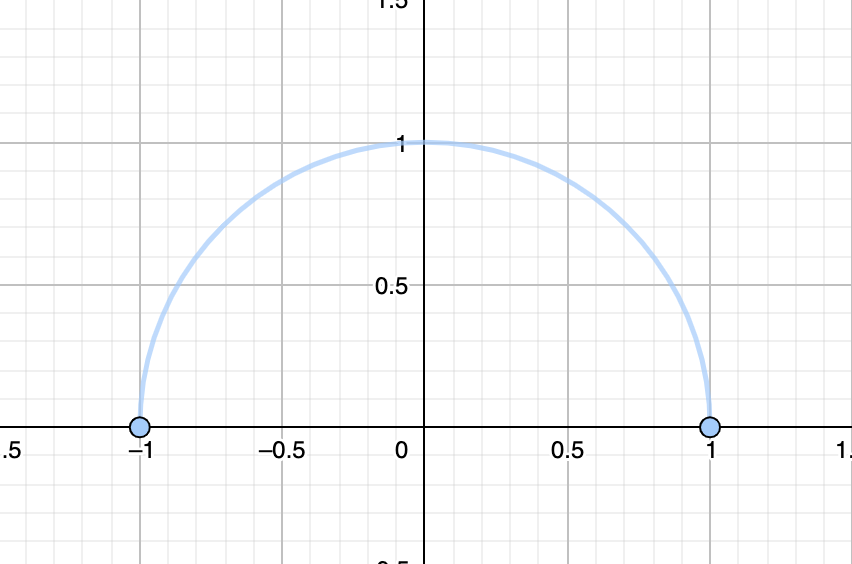
\includegraphics[width=50mm]{X_n1_2.png}
         \caption{$S_{+}^{1} = \{ (x_1, x_2)\in S^1 \ ; \ x_{2} \geq 0\}$.}
    \end{minipage}\hfill
    \begin{minipage}{0.5\textwidth}
         \centering
         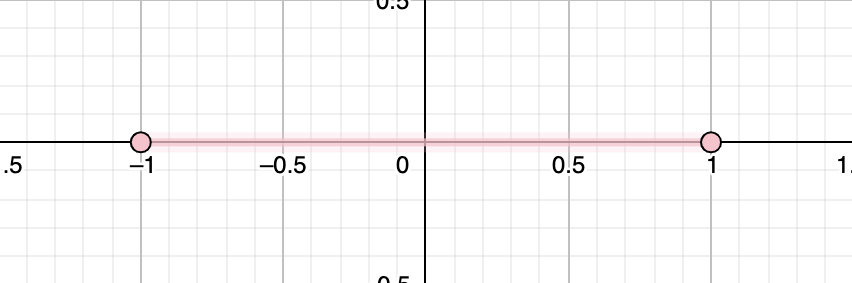
\includegraphics[width=70mm]{Y_n1_2.png}
         \caption{$B^1 = \{ x_1 \in \mathbb{R} \ ; \_1^2  \leq 1\}$.}
    \end{minipage}\hfill
\end{figure}
\noindent
To get from left to right, the idea is to project the circle down on the line (so we no longer use coordinate $x_2$ and coordinate $x_1$ stays the same), and from right to left to stretch the line up to circle (we add the new coordinate $x_2$ as a function of $x_1$). 

\begin{figure}[ht]
    \begin{minipage}{0.5\textwidth}
         \centering
         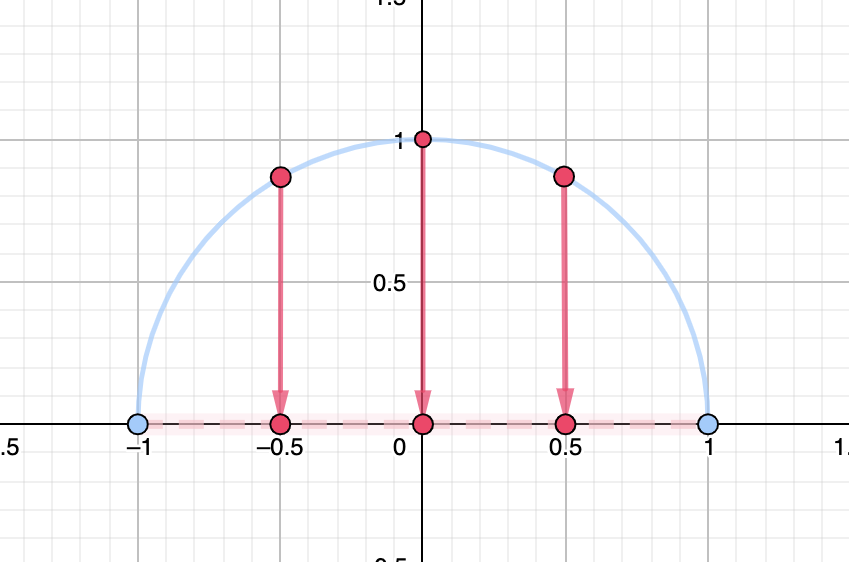
\includegraphics[width=70mm]{XY_2.png}
         \caption{The idea for function $S_{+}^{1} \to B^1$.}
    \end{minipage}\hfill
    \begin{minipage}{0.5\textwidth}
         \centering
         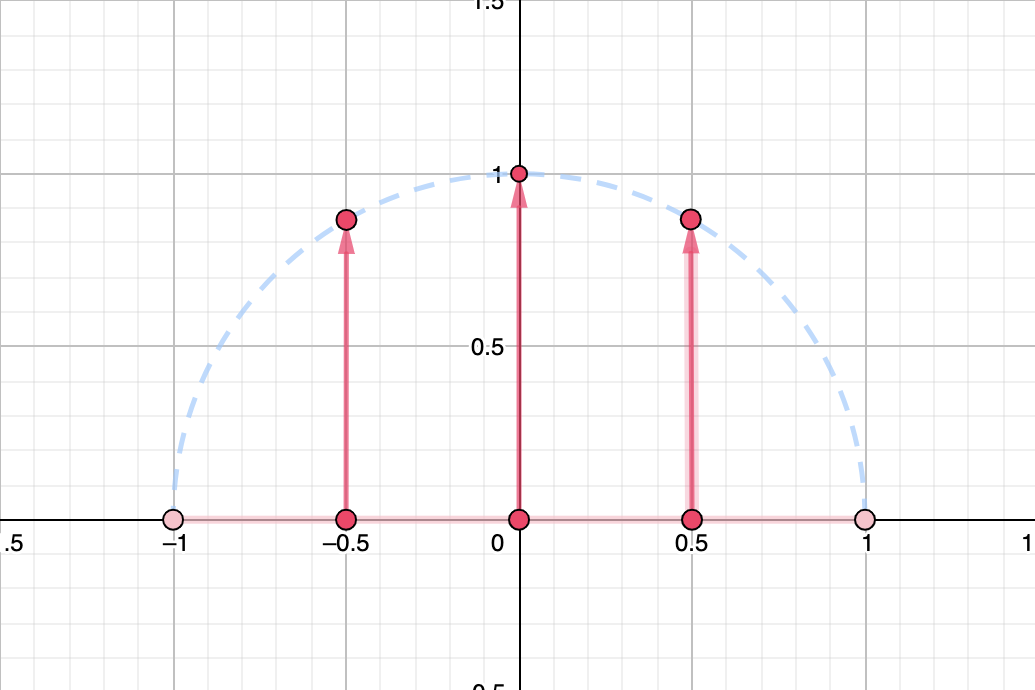
\includegraphics[width=70mm]{YX_2.png}
         \caption{The idea for function $B^1 \to S_{+}^{1}$.}
    \end{minipage}\hfill
\end{figure}
\noindent
Using that idea, we write the regulation for general n.
\\
Let $f: S_{+}^{n} \subset \mathbb{R}^{n + 1} \to B^n \subset \mathbb{R}^n$ and let $g: B^n \in \mathbb{R}^n \to S_{+}^{n} \in \mathbb{R}^{n + 1}$. 
\\
\\
As said before, to determine function $f$, we just skip the last coordinate.
$$ f(x_1, x_2, \ldots, x_{n + 1}) = (x_1, x_2, \ldots, x_n). $$

\noindent
We need to check if $(x_1, \ldots, x_n) \in B^n$. For $(x_1, x_2, \ldots, x_{n + 1}) \in S_{+}^{n}$ the relations $x_1^2 + \cdots + x_n^2 + x_{n + 1}^2 = 1$ and $x_{n+1} \in [0,1]$ are valid and that implies that $x_1^2 + \cdots + x_n^2 = 1 - x_{n+1}^2 \leq 1$, so the condition is satisfied.
\\
\\
For function $g$ we need to express the new coordinate $x_{n + 1}$ as a function of $(x_1, \ldots, x_n)$.
We get $x_{n + 1} = \sqrt{ 1 - x_1^2 - \cdots - x_n^2}$ (we take the positive root because we are in the $S_{+}^{n}$). 

$$ g(x_1, \ldots, x_n) = \left( x_1, \ldots, x_n, \sqrt{ 1 - x_1^2 - \cdots - x_n^2} \right). $$

\noindent
We need to check if $\left( x_1, \ldots, x_n, \sqrt{ 1 - x_1^2 - \cdots - x_n^2} \right) \in S_{+}^{n}$. For $(x_1, \ldots, x_n) \in B^n$ the relation $x_1^2 + \cdots x_n^2 \leq 1 $ is true and $x_1^2 + \cdots + x_n^2 + x_{n + 1}^2 = x_1^2 + \cdots + x_n^2 + 1 - x_1^2 - \cdots - x_n^2 = 1$, so $x_{n+1} \geq 0$ and the condition is satisfied.
\\
Clearly, both function are continuous. 
\\
All there is left to do is to calculate both compositums, which are continuous, too.

$$ (f \circ g): B^n \to S_{+}^{n} \to B^n $$
$$ (f \circ g)(x_1, \ldots, x_n) = f \left(x_1, \ldots, x_n, \sqrt{ 1 - x_1^2 - \cdots - x_n^2} \right) = (x_1, \ldots, x_n) = \text{id}_{B^n}$$
\\
$$ (g \circ f): S_{+}^{n} \to B^n \to S_{+}^{n} $$
$$ (g \circ f)(x_1, \ldots, x_n, x_{n + 1}) = g(x_1, \ldots, x_n) = \left(x_1, \ldots, x_n, \sqrt{ 1 - x_1^2 - \cdots - x_n^2} \right) = (x_1, \ldots, x_n, x_{n + 1}) = \text{id}_{S_{+}^{n}}$$
\noindent
$ \Longrightarrow S_{+}^{n} \cong B^n.$

\section{Programming problems}


\end{document}